\documentclass{article}
\usepackage{arxiv}
\usepackage[T1]{fontenc}
\usepackage{amsfonts}
\usepackage{amsmath,amssymb,amsthm}
\usepackage{nicefrac}
\usepackage{microtype}
\usepackage{graphicx}
\usepackage{float}
\usepackage{subcaption}
\usepackage{booktabs}
\usepackage{xcolor}
\usepackage{pgfplots}
\pgfplotsset{compat=1.16}
\usepackage[numbers,sort&compress]{natbib}
\usepackage{url}
\usepackage{pdfpages}
\usepackage{listings}
\lstset{%
  basicstyle=\small\ttfamily,
  breaklines=true,
  breakatwhitespace=true,
  breakindent=0pt,
  columns=fullflexible,
  keepspaces=true,
  frame=single,
  showstringspaces=false,
  xleftmargin=3pt,
  xrightmargin=3pt,
  framexleftmargin=0pt,
  framexrightmargin=0pt,
  linewidth=\dimexpr\linewidth-6pt-2\fboxsep-2\fboxrule\relax,
  aboveskip=0.6\baselineskip,
  belowskip=0.6\baselineskip
}
\usepackage{hyperref}  % load last
\hypersetup{hidelinks}
\graphicspath{ {./images/} }

\newcommand{\modelA}{Qwen2.5-7B-Instruct}
\newcommand{\repourl}{https://github.com/Fakharalamkhan/confidence-gated-self-correction}
\newtheorem{proposition}{Proposition}

\title{Knowing When to Revise: Confidence-Gated Self-Correction in Large Language Models}
\author{
  Fakhr E Alam Khan \\
  University of Trier \\
  Trier, Germany \\
  Matriculation No.\ 1818211 \\
  \texttt{s2fakhan@uni-trier.de} \\
  {\small\url{\repourl}}
}

\begin{document}
\maketitle
\begin{abstract}
Intrinsic self-correction means asking a large language model to critique and revise its own answer without external feedback. It often fails to improve accuracy, because revision can turn correct answers into incorrect ones. One possible fix is confidence gating: revise only when the model's confidence in its initial answer is low. We give a simple analytical model of gated revision. It shows that the gain of any gate is capped by how often the revision step repairs a wrong answer, and that an uninformative signal can never beat the better of never and always revising. We then compare three training-free confidence signals (verbalised confidence, self-consistency and P(True) self-verification) as gates for \modelA{} on GSM8K and HotpotQA, with thresholds tuned on a development split. Self-critique almost never repairs an error (fix rate 0 on GSM8K, 0.04 on HotpotQA), so no gate improves on never revising. Self-consistency, however, identifies wrong answers well (AUROC 0.95 on GSM8K), and its majority answer repairs 47\% of GSM8K errors; used as the revision step, the same gates behave as the analytical model predicts. The results suggest that the bottleneck of self-correction is the revision step, not the decision of when to revise.
\end{abstract}

\keywords{Large Language Models \and Intrinsic Self-Correction \and Confidence Estimation \and Selective Revision \and Test-Time Compute}
\section{Introduction}
\label{sec:introduction}

A common way to get more out of a large language model (LLM) at inference time is to let it check its own work. The model first produces an answer $A_0$, then critiques that answer, and finally writes a revised answer $A_1$. Self-Refine~\cite{madaan2023selfrefine} and Reflexion~\cite{shinn2023reflexion} made this loop popular, and it is now a standard building block of LLM pipelines. In this paper we study the \emph{intrinsic} version of the loop, in which the model receives no outside help: no code execution, no retrieval, and no ground-truth checker tells it whether $A_0$ was right.

Whether intrinsic self-correction actually helps is disputed. Huang et al.~\cite{huang2024cannot} found that once the oracle signal that earlier work used to decide when to stop is removed, revision on reasoning benchmarks often lowers accuracy. A survey by Kamoi et al.~\cite{kamoi2024when} concludes that reliable intrinsic self-correction has so far been shown only in narrow settings, and Stechly et al.~\cite{stechly2023gpt4} report that models are poor judges of their own solutions. The reason becomes clear once each revision is tracked individually. A revision step turns some wrong answers into right ones ($W\to R$), but it also turns some right answers into wrong ones ($R\to W$). When initial accuracy is high, there are many more correct answers that can be damaged than wrong answers that can be repaired, so even a small break rate can cancel the benefit. A single net-accuracy number hides this, because a small gain can be the sum of many fixes and many breaks.

A simple response is to revise only when the model is unsure. We call this \emph{confidence-gated self-correction}. A confidence score $S(A_0)$ is computed for the initial answer, and the revised answer is used if and only if $S(A_0)<\tau$ for a threshold $\tau$; otherwise $A_0$ is kept.

Li et al.~\cite{li2024confidence} already proposed the If-or-Else (IoE) prompt, which asks the model to keep its answer if it is confident and to revise it otherwise. In this way the decision is made inside a single prompt. Yang et al.~\cite{yang2024confidence} split self-correction into a confidence ability (keeping answers that are already correct) and a critique ability (fixing answers that are wrong). They showed that the two can trade off against each other. However, two questions are still open. First, it is not clear when gating can help at all, and how large the gain can be for a given revision step and confidence signal. Second, there is no controlled comparison of different confidence signals used as explicit threshold gates, with thresholds chosen on held-out data and with the cost of computing each signal taken into account.

This paper addresses both gaps. The study is organised around three research questions:
\begin{itemize}
    \item \textbf{RQ1 (Gating efficacy):} Does confidence gating outperform both never revising and always revising on held-out data, and how close does it come to an oracle gate?
    \item \textbf{RQ2 (Signal discrimination):} Which training-free confidence signal best separates correct from incorrect initial answers?
    \item \textbf{RQ3 (Accuracy--cost trade-off):} How does the cost of computing each signal, split into prefill and completion tokens, change the trade-off between accuracy and compute?
\end{itemize}

\paragraph{Contributions.} This paper makes three contributions.
\begin{itemize}
    \item \textbf{An analytical model of gated revision} (Section~\ref{sec:theory}). We express the accuracy of a gated system in closed form, in terms of the initial accuracy, the fix and break rates of the revision step, and the operating point of the confidence signal on its ROC curve. From this we derive when gating beats never and always revising, and show that an uninformative signal can never beat the better of the two. The model also locates the optimal threshold at a fixed slope of the ROC curve and bounds the achievable gain by the fix rate. Finally, it explains why a high AUROC alone does not guarantee a large gain.
    \item \textbf{A controlled comparison of confidence signals.} We compare three training-free signals (verbalised confidence, self-consistency agreement and P(True) self-verification) on GSM8K and HotpotQA with \modelA{}~\cite{qwen2025qwen25}. Thresholds are tuned on a development split and applied once to a test split. Differences are tested with exact McNemar tests, and the baselines include IoE, majority voting and an oracle gate.
    \item \textbf{A transition and cost analysis.} Every revision is broken down into its four possible outcomes, and cost is measured with a token model that separates prefill from completion tokens. We also inspect the $R\to W$ failures and separate changes in answer form from changes in content.
\end{itemize}
With \modelA{}, self-critique almost never fixes an error, so no gate beats never revising. Self-consistency, in contrast, identifies wrong answers well and, when used as the revision step, repairs many of them. With that revision step, gated accuracy matches the analytical model closely.

The rest of the paper is organised as follows. Section~\ref{sec:related_work} reviews related work, Section~\ref{sec:theory} presents the analytical model, Section~\ref{sec:methodology} describes the experimental setup, Section~\ref{sec:experiments} reports the results, Section~\ref{sec:analysis} analyses them in more depth. Sections~\ref{sec:discussion} and~\ref{sec:limitations} discuss implications and limitations, and Section~\ref{sec:conclusion} concludes.

\section{Related Work}
\label{sec:related_work}

\paragraph{Self-correction without external feedback.}
Self-Refine~\cite{madaan2023selfrefine} uses one model in three roles (generator, critic and reviser) and iterates between them without any additional training. Reflexion~\cite{shinn2023reflexion} lets an agent write verbal reflections on the feedback it received for a task and keeps them in memory for later attempts. Both reported gains on a range of tasks, but later work questioned how much of the gain comes from the model itself. Huang et al.~\cite{huang2024cannot} showed that on GSM8K, CommonSenseQA and HotpotQA, part of the reported improvement came from using the ground-truth label to decide when to stop, and that purely intrinsic self-correction frequently made answers worse. Stechly et al.~\cite{stechly2023gpt4} studied iterative prompting of GPT-4 on graph colouring and found its self-critiques unreliable; most of the improvement came from a correct answer happening to appear among several candidates rather than from the critique itself. Kamoi et al.~\cite{kamoi2024when} reviewed the field and concluded that self-correction works reliably when trustworthy external feedback is available or when the model is fine-tuned for it, but that there is little evidence of success with prompting alone. Starting from this picture, we ask a narrower question: given a revision step that sometimes helps and sometimes hurts, can we decide in advance which answers to revise?

\paragraph{Confidence estimation for LLMs.}
A gate needs a confidence score, and several training-free ways to obtain one exist. The simplest is to ask the model directly. Xiong et al.~\cite{xiong2024can} evaluated such verbalised confidence together with sampling-based and hybrid methods across several models. They found that verbalised scores tend to be overconfident, and that checking consistency across multiple responses helps to reduce this. Self-consistency~\cite{wang2023selfconsistency} samples several reasoning paths and returns the majority answer; the share of samples that agree with a given answer is a simple measure of how sure the model is. Kadavath et al.~\cite{kadavath2022language} asked models to judge whether a proposed answer is true and read off the probability of ``True'', known as P(True); they found that larger models are well calibrated when questions are posed in a suitable format. We compare these three families of signals: verbalised, sampling-based and probability-based. Prior work mostly evaluates them as predictors of correctness, while we evaluate them as decision rules for whether to revise.

\paragraph{Confidence and self-correction.}
Two recent papers connect confidence directly to revision. Li et al.~\cite{li2024confidence} identify the model's confidence as a key hidden factor in intrinsic self-correction and propose the IoE prompt, in which the model assesses its own confidence and decides in the same prompt whether to keep or revise its answer. Yang et al.~\cite{yang2024confidence} define probabilistic measures for the confidence and critique abilities, report a trade-off between them under prompting, and propose a fine-tuning data format that improves both. The present study differs from these in three respects. First, the gate is an explicit threshold on a separately computed score rather than a decision left to the revision prompt, so different signals can be swapped in and compared under one protocol. Second, thresholds are selected on a development split and evaluated once on a test split. Third, an analytical model links the ROC curve of a signal to the accuracy gain it can deliver and explains when and why gating helps.

\section{An Analytical Model of Confidence-Gated Revision}
\label{sec:theory}

Before running any experiment, it helps to ask what a confidence gate can and cannot achieve. The small model in this section answers the question with a few quantities that can all be measured on real data.

\paragraph{Setup.} Consider one question. Let $Y_0\in\{0,1\}$ indicate whether the initial answer $A_0$ is correct, let $Y_1\in\{0,1\}$ indicate whether the revised answer $A_1$ is correct, and let $S$ be a confidence score computed from $A_0$. We describe the revision step by three numbers:
\begin{align*}
a &= P(Y_0=1) && \text{initial accuracy,}\\
f &= P(Y_1=1 \mid Y_0=0) && \text{fix rate: how often revision repairs a wrong answer,}\\
b &= P(Y_1=0 \mid Y_0=1) && \text{break rate: how often revision damages a right answer.}
\end{align*}
A gate with threshold $\tau$ revises when $S<\tau$. Since the gate should catch wrong answers, we treat ``$A_0$ is wrong'' as the positive class. The gate then has a true-positive rate $t(\tau)=P(S<\tau\mid Y_0=0)$, the share of wrong answers it sends to revision, and a false-positive rate $u(\tau)=P(S<\tau\mid Y_0=1)$, the share of right answers it sends to revision. As $\tau$ varies, the pair $(u,t)$ traces the ROC curve of the signal~\cite{fawcett2006roc}.

\paragraph{Assumption.} We assume that, once we know whether $A_0$ is correct, the outcome of the revision does not depend on the confidence score: $Y_1 \perp S \mid Y_0$. This is a simplification. A model that is unsure about an answer may also be worse at fixing it, which would make the fix rate lower among low-confidence answers. We test how much this matters in Section~\ref{sec:assumption}.

\paragraph{Gated accuracy.} Under this assumption, a correct answer is lost only if the gate sends it to revision and the revision breaks it, and a wrong answer is recovered only if the gate sends it to revision and the revision fixes it. The accuracy of the gated system is then
\begin{equation}
\mathrm{Acc}(\tau) \;=\; a \;+\; (1-a)\,f\,t(\tau) \;-\; a\,b\,u(\tau).
\label{eq:gated}
\end{equation}
The three reference systems are special points of this formula. Never revising is $(u,t)=(0,0)$ with accuracy $a$. Always revising is $(u,t)=(1,1)$ with accuracy $a+(1-a)f-ab$. The oracle gate, which revises exactly the wrong answers, is $(u,t)=(0,1)$ with accuracy $a+(1-a)f$.

\paragraph{When does gating pay off?} Define the damage-to-repair ratio
\begin{equation}
\kappa \;=\; \frac{a\,b}{(1-a)\,f},
\end{equation}
the expected number of correct answers broken for every wrong answer fixed when all answers are revised. Always revising improves on never revising if and only if $\kappa<1$. Rearranging Eq.~\eqref{eq:gated}, a gate operating at $(u,t)$ beats never revising if and only if
\begin{equation}
\frac{t}{u} \;>\; \kappa,
\label{eq:beat_never}
\end{equation}
and beats always revising if and only if
\begin{equation}
\frac{1-u}{1-t} \;>\; \frac{1}{\kappa}.
\label{eq:beat_always}
\end{equation}
So, to beat never revising, the gate must send wrong answers to revision at least $\kappa$ times as often as right ones. To beat always revising, it must hold back right answers at least $1/\kappa$ times as often as wrong ones.

\begin{proposition}[No free gating]
\label{prop:nofree}
If the confidence signal is uninformative, i.e.\ $t(\tau)=u(\tau)$ for every $\tau$, then for every threshold the gated accuracy lies between the accuracies of never and always revising. As a consequence, an uninformative gate can never beat the better of the two baselines.
\end{proposition}
\noindent\textit{Proof.} Setting $t=u=q$ in Eq.~\eqref{eq:gated} gives $\mathrm{Acc}=a+q\,[(1-a)f-ab]$. This is linear in $q\in[0,1]$, equals the never-revise accuracy at $q=0$ and the always-revise accuracy at $q=1$, and so never leaves the interval between them. $\square$

\paragraph{The optimal threshold.} Eq.~\eqref{eq:gated} is linear in $(u,t)$, so lines of equal accuracy are straight lines of slope $\kappa$ in ROC space. The best threshold is the point at which the ROC curve has slope $\kappa$, the same result as in cost-sensitive ROC analysis~\cite{fawcett2006roc}. When revision is harmful on average ($\kappa>1$), this point lies close to the origin: the gate should revise only a small set of answers for which the signal is quite sure that $A_0$ is wrong.

\paragraph{A ceiling on the gain.} Because $t\le 1$ and $u\ge 0$, the gain of any gate over never revising is at most $(1-a)f$, which is exactly the gain of the oracle gate. If the revision step rarely fixes errors, even a perfect signal can deliver only a small improvement. A gate can remove harm, but it cannot create fixes.

\paragraph{Why AUROC is not enough.} AUROC summarises the whole ROC curve, but by Eq.~\eqref{eq:gated} only the part of the curve near slope $\kappa$ determines the gain. As a result, two signals with the same AUROC can give different gains, and a signal with a high AUROC gives little benefit when the fix rate $f$ is small. For this reason we report both the AUROC of each signal and the accuracy gain it actually achieves.

\paragraph{Illustration.} Figure~\ref{fig:theory} evaluates Eq.~\eqref{eq:gated} for hypothetical values $a=0.80$, $b=0.15$ and $f=0.30$. Here $\kappa=2$, so always revising costs 6 points, and the oracle ceiling is $(1-a)f=6$ points. We model the signal with equal-variance binormal ROC curves of separation $d'$. An uninformative signal ($d'=0$) only moves along the straight line between the two baselines, as Proposition~\ref{prop:nofree} states. A signal with AUROC $0.76$ ($d'=1$) gains at most about 1.1 points, one with AUROC $0.92$ ($d'=2$) about 3.4 points, and one with AUROC $0.98$ ($d'=3$) about 4.9 points, still below the ceiling. In every case the best operating point revises fewer than 12\% of the correct answers.

\begin{figure}[t]
\centering
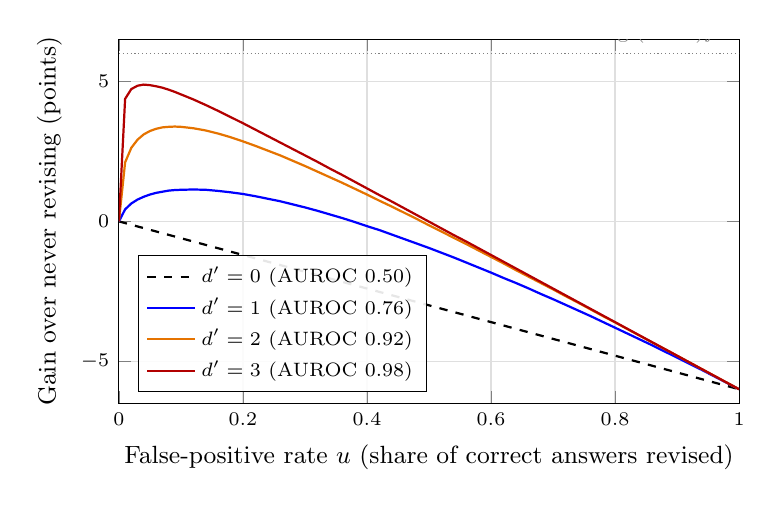
\begin{tikzpicture}
\begin{axis}[
  width=0.78\linewidth, height=6.2cm,
  xlabel={False-positive rate $u$ (share of correct answers revised)},
  ylabel={Gain over never revising (points)},
  xmin=0, xmax=1, ymin=-6.5, ymax=6.5,
  grid=major, grid style={gray!25},
  legend pos=south west, legend style={font=\scriptsize, fill=white, fill opacity=0.9, text opacity=1},
  tick label style={font=\scriptsize}, label style={font=\small},
]
\addplot[thick, dashed, black] coordinates {(0,0) (1,-6)};
\addlegendentry{$d'=0$ (AUROC 0.50)}
\addplot[thick, blue] coordinates {(0.000,0.00) (0.010,0.43) (0.020,0.64) (0.030,0.78) (0.040,0.88) (0.050,0.96) (0.060,1.02) (0.070,1.06) (0.080,1.10) (0.090,1.12) (0.100,1.13) (0.120,1.14) (0.140,1.13) (0.160,1.09) (0.180,1.04) (0.200,0.98) (0.220,0.90) (0.240,0.81) (0.260,0.72) (0.280,0.61) (0.300,0.50) (0.320,0.38) (0.340,0.25) (0.360,0.12) (0.380,-0.02) (0.400,-0.17) (0.420,-0.31) (0.440,-0.47) (0.460,-0.63) (0.480,-0.79) (0.500,-0.95) (0.520,-1.12) (0.540,-1.29) (0.560,-1.47) (0.580,-1.65) (0.600,-1.83) (0.620,-2.02) (0.640,-2.20) (0.660,-2.39) (0.680,-2.59) (0.700,-2.78) (0.720,-2.98) (0.740,-3.18) (0.760,-3.38) (0.780,-3.59) (0.800,-3.80) (0.820,-4.01) (0.840,-4.22) (0.860,-4.43) (0.880,-4.65) (0.900,-4.87) (0.920,-5.09) (0.940,-5.31) (0.960,-5.54) (0.980,-5.77) (1.000,-6.00)};
\addlegendentry{$d'=1$ (AUROC 0.76)}
\addplot[thick, orange!90!black] coordinates {(0.000,0.00) (0.010,2.11) (0.020,2.63) (0.030,2.92) (0.040,3.11) (0.050,3.23) (0.060,3.31) (0.070,3.36) (0.080,3.38) (0.090,3.39) (0.100,3.38) (0.120,3.33) (0.140,3.25) (0.160,3.14) (0.180,3.01) (0.200,2.86) (0.220,2.70) (0.240,2.53) (0.260,2.36) (0.280,2.17) (0.300,1.98) (0.320,1.78) (0.340,1.58) (0.360,1.38) (0.380,1.17) (0.400,0.96) (0.420,0.74) (0.440,0.53) (0.460,0.31) (0.480,0.09) (0.500,-0.14) (0.520,-0.36) (0.540,-0.59) (0.560,-0.81) (0.580,-1.04) (0.600,-1.27) (0.620,-1.50) (0.640,-1.74) (0.660,-1.97) (0.680,-2.20) (0.700,-2.43) (0.720,-2.67) (0.740,-2.90) (0.760,-3.14) (0.780,-3.38) (0.800,-3.61) (0.820,-3.85) (0.840,-4.09) (0.860,-4.33) (0.880,-4.56) (0.900,-4.80) (0.920,-5.04) (0.940,-5.28) (0.960,-5.52) (0.980,-5.76) (1.000,-6.00)};
\addlegendentry{$d'=2$ (AUROC 0.92)}
\addplot[thick, red!70!black] coordinates {(0.000,0.00) (0.010,4.38) (0.020,4.73) (0.030,4.85) (0.040,4.89) (0.050,4.87) (0.060,4.83) (0.070,4.78) (0.080,4.71) (0.090,4.63) (0.100,4.54) (0.120,4.36) (0.140,4.16) (0.160,3.95) (0.180,3.73) (0.200,3.51) (0.220,3.28) (0.240,3.05) (0.260,2.82) (0.280,2.59) (0.300,2.36) (0.320,2.13) (0.340,1.89) (0.360,1.66) (0.380,1.42) (0.400,1.18) (0.420,0.94) (0.440,0.71) (0.460,0.47) (0.480,0.23) (0.500,-0.01) (0.520,-0.25) (0.540,-0.49) (0.560,-0.72) (0.580,-0.96) (0.600,-1.20) (0.620,-1.44) (0.640,-1.68) (0.660,-1.92) (0.680,-2.16) (0.700,-2.40) (0.720,-2.64) (0.740,-2.88) (0.760,-3.12) (0.780,-3.36) (0.800,-3.60) (0.820,-3.84) (0.840,-4.08) (0.860,-4.32) (0.880,-4.56) (0.900,-4.80) (0.920,-5.04) (0.940,-5.28) (0.960,-5.52) (0.980,-5.76) (1.000,-6.00)};
\addlegendentry{$d'=3$ (AUROC 0.98)}
\addplot[thin, gray, densely dotted] coordinates {(0,6) (1,6)};
\node[font=\scriptsize, gray, anchor=south east] at (axis cs:0.98,6) {oracle ceiling $(1-a)f$};
\end{axis}
\end{tikzpicture}
\caption{Gain of confidence gating over never revising, as a function of the share of correct answers that are revised, computed from Eq.~\eqref{eq:gated} with hypothetical parameters $a=0.80$, $b=0.15$, $f=0.30$ and binormal ROC curves of separation $d'$. The right end ($u=1$) corresponds to always revising ($-6$ points). The figure illustrates the model only; it does not show experimental data.}
\label{fig:theory}
\end{figure}

\section{Experimental Setup}
\label{sec:methodology}

\subsection{Tasks, Data and Scoring}
We use two tasks with short answers that can be checked automatically. \textbf{GSM8K}~\cite{cobbe2021gsm8k} consists of grade-school math word problems whose answer is a single number. \textbf{HotpotQA}~\cite{yang2018hotpotqa} consists of multi-hop questions over Wikipedia. In its distractor setting, each question comes with two gold paragraphs and eight distractor paragraphs, and all ten paragraphs are given to the model. The data are 500 questions from the GSM8K test set and 500 from the HotpotQA validation set, sampled with seed 42. Each dataset is randomly split (seed 42) into a development split $D_{\text{dev}}$ with 20\% of the questions, used only to choose thresholds, and a test split $D_{\text{test}}$ with the remaining 80\%, used once for all reported results.

Every prompt that produces an answer asks the model to finish with a line of the form \texttt{Final answer: <answer>}, and only this span is scored. For GSM8K we extract the number, remove formatting such as commas, currency signs and trailing zeros, and compare it with the gold number. For HotpotQA we apply the official answer normalisation (lower-casing and removing punctuation, articles and extra whitespace) and compute exact match (EM) and token-level F1. The correctness label $Y$ is EM on the extracted answer. To measure how much apparent harm is caused only by changes in answer form, we also use a \emph{lenient match}, which counts an answer as correct if the normalised gold answer is contained in the normalised extracted answer.

\subsection{Models and Inference}
We use the open instruction-tuned model \modelA{}~\cite{qwen2025qwen25} with its own chat template, served with vLLM 0.6.6.post1 on two NVIDIA T4 GPUs (16\,GB each) in 16-bit floating point. The initial answer, the revision and the IoE baseline use greedy decoding, so the only randomness in the pipeline comes from the self-consistency samples, each of which is drawn with its own random seed.

\subsection{Pipeline and Confidence Signals}
For each question we first generate the initial answer $A_0$. We then compute three confidence scores $S(A_0)\in[0,1]$, each in a separate call so that one signal cannot influence another. The full prompts are listed in Appendix~\ref{app:prompts}.
\begin{enumerate}
    \item \textbf{Verbalised confidence $S_{\text{verb}}$.} In a new turn after $A_0$, the model is asked to state how confident it is that its final answer is correct, as a whole number from 0 to 100, which we divide by 100. If the reply cannot be parsed, we set $S_{\text{verb}}=1$, so that the answer is never revised by this gate, and we report the number of such cases.
    \item \textbf{Self-consistency agreement $S_{\text{sc}}$.} We draw $N=10$ additional samples with the same prompt as $A_0$, at temperature $0.7$ and top-$p$ $0.95$. With $k$ the number of samples whose normalised extracted answer equals that of $A_0$, we set $S_{\text{sc}}=k/N$. We also report the variant with $N=5$, which uses the first five samples.
    \item \textbf{Self-verification $S_{\text{verif}}$ (P(True)).} Following Kadavath et al.~\cite{kadavath2022language}, the model sees the question (for HotpotQA also the ten paragraphs) together with the extracted answer of $A_0$, and must choose between ``(A) True'' and ``(B) False''. With $p_A$ and $p_B$ the next-token probabilities of the two options, summed over their tokenisation variants, we set $S_{\text{verif}}=p_A/(p_A+p_B)$. The gold answer never appears in this prompt.
\end{enumerate}
Finally, the model revises $A_0$ in the same conversation with a fixed critique-and-revise prompt, producing $A_1$. The revision is computed for every question, whatever its confidence. This lets us evaluate all gating policies offline on exactly the same outputs, so differences between policies come only from the decision of whether to revise.

Table~\ref{tab:signals} summarises what each signal needs. The signals differ in two practical ways: whether they require access to token probabilities, and whether their cost comes mainly from reading the input (prefill) or from generating text (completion).

\begin{table}[h!]
\caption{The three confidence signals and what they require per question, in addition to generating $A_0$.}
\centering
\small
\begin{tabular}{lcccc}
\toprule
Signal & Extra calls & Token probabilities & Main cost & Output \\
\midrule
$S_{\text{verb}}$  & 1  & not needed & short completion & integer 0--100 \\
$S_{\text{sc}}$    & 10 & not needed & 10 full completions & agreement $k/N$ \\
$S_{\text{verif}}$ & 1  & needed     & prefill (question and context) & $p_A/(p_A+p_B)$ \\
\bottomrule
\end{tabular}
\label{tab:signals}
\end{table}

\subsection{Gating, Baselines and Threshold Selection}
A gate with signal $S$ and threshold $\tau$ outputs $A_1$ if $S(A_0)<\tau$ and $A_0$ otherwise. We evaluate gates on $S_{\text{verb}}$, $S_{\text{sc}}$ and $S_{\text{verif}}$, and on the simple combination $S_{\text{avg}}=\tfrac12(S_{\text{verb}}+S_{\text{sc}})$, which, like its two parts, needs no access to token probabilities. For each gate, the threshold $\tau^*$ is chosen on $D_{\text{dev}}$ among all observed score values as the one with the highest dev accuracy; ties are broken in favour of the threshold that revises fewer questions. The chosen $\tau^*$ is then applied once to $D_{\text{test}}$.

We compare the gates against five baselines:
\begin{itemize}
    \item \textbf{Never revise:} output $A_0$.
    \item \textbf{Always revise:} output $A_1$.
    \item \textbf{Majority vote:} output the most frequent extracted answer among $A_0$ and the ten self-consistency samples, a strong baseline that uses the same samples as $S_{\text{sc}}$.
    \item \textbf{IoE}~\cite{li2024confidence}: a single revision prompt that tells the model to keep its answer if it is confident and to change it otherwise, using the prompt of the original paper.
    \item \textbf{Oracle gate:} revise exactly the questions for which $A_0$ is wrong. It uses the gold labels and serves only as an upper bound, not as a practical method.
\end{itemize}

\paragraph{Majority vote as a revision step.} To test the analytical model with a revision step that does repair errors, we also use the majority answer over the ten self-consistency samples, denoted $R_{\text{mv}}$, in place of $A_1$, and gate it with $S_{\text{sc}}$ and $S_{\text{avg}}$ in exactly the same way. This needs no additional model calls, because the samples are already computed for $S_{\text{sc}}$.

\subsection{Metrics and Cost Model}
\textbf{Transitions.} Each question falls into one of four cells: $W\to R$ ($Y_0=0$, $Y_1=1$), $R\to W$ ($Y_0=1$, $Y_1=0$), $R\to R$ or $W\to W$. For a gated method, only the questions it revises can change cell. From the always-revise transitions we estimate $a$, $f$, $b$ and $\kappa$ as defined in Section~\ref{sec:theory}.

\textbf{Discrimination.} For each signal we report the AUROC for predicting $Y_0=1$ on $D_{\text{test}}$, with 95\% confidence intervals from 1{,}000 bootstrap resamples of the test questions.

\textbf{Significance.} Two methods are evaluated on the same questions, so we compare their accuracies with the exact (binomial) McNemar test on the discordant pairs, against both never revising and always revising. We report exact $p$-values rather than significance stars.

\textbf{Cost.} For question $i$ and a gated method we count
\begin{equation}
C_i \;=\; C_i^{A_0} \;+\; C_i^{S} \;+\; \mathbb{1}[S_i<\tau]\;C_i^{\text{rev}},
\label{eq:cost}
\end{equation}
where $C_i^{A_0}$, $C_i^{S}$ and $C_i^{\text{rev}}$ are the tokens used for the initial answer, for computing the signal and for the revision. We keep prompt (prefill) tokens and generated (completion) tokens separate. Prefill matters here because the verification and revision calls re-read the question and, for HotpotQA, all ten paragraphs. For majority voting the cost is the initial answer plus the ten samples.

\section{Results}
\label{sec:experiments}

\subsection{Unguided Revision}
\begin{table}[ht]
\centering
\caption{Outcome of unguided (always) revision on the test set ($N=400$ per dataset). We report initial accuracy $\text{Acc}(A_0)$, transition frequencies ($W\to R$, $R\to W$, $R\to R$, $W\to W$), accuracy delta $\Delta = \text{Acc}(A_1) - \text{Acc}(A_0)$, empirical fix rate $f$, break rate $b$, base accuracy $a$, and the gating threshold ratio $\kappa = \frac{a b}{(1-a)f}$.}
\label{tab:transitions}
\resizebox{\linewidth}{!}{\begin{tabular}{llcccccccccc}
\toprule
Model & Dataset & $N$ & Acc($A_0$) & $W\to R$ & $R\to W$ & $R\to R$ & $W\to W$ & $\Delta$ & $f$ & $b$ & $\kappa$ \\
\midrule
\modelA{} & GSM8K & 400 & 92.5\% & 0 (0.0\%) & 1 (0.3\%) & 369 (92.3\%) & 30 (7.5\%) & -0.3\% & 0.000 & 0.003 & $\infty$ \\
\modelA{} & HotpotQA & 400 & 58.8\% & 6 (1.5\%) & 21 (5.3\%) & 214 (53.5\%) & 159 (39.8\%) & -3.8\% & 0.036 & 0.089 & 3.50 \\
\bottomrule
\end{tabular}
}
\end{table}

Table~\ref{tab:transitions} shows what happens when every answer is revised. On GSM8K, \modelA{} starts at 92.5\% accuracy and revision changes almost nothing: on the 400 test questions it fixes no wrong answer and breaks one correct answer, so accuracy moves to 92.25\%. On HotpotQA revision is clearly harmful: it breaks 21 correct answers and fixes only 6, which lowers accuracy from 58.75\% to 55.0\% (exact McNemar test against never revising, $p=0.006$). In the terms of Section~\ref{sec:theory}, GSM8K has a fix rate of $f=0$, so the oracle ceiling $(1-a)f$ is zero. HotpotQA has $f=0.036$ and $b=0.089$, giving $\kappa=3.5$: revision damages about 3.5 correct answers for every wrong answer it repairs, and even a perfect gate could gain at most 1.5 points.

\subsection{Signal Discrimination (RQ2)}
\begin{table}[ht]
\centering
\caption{AUROC with 95\% bootstrap confidence intervals for predicting initial answer correctness $Y_0=1$ on the test set ($N=400$ per dataset). Higher values indicate stronger discrimination.}
\label{tab:auroc}
\resizebox{\linewidth}{!}{\begin{tabular}{llccccc}
\toprule
Model & Dataset & $S_{\text{verb}}$ & $S_{\text{sc5}}$ & $S_{\text{sc10}}$ & $S_{\text{verif}}$ & $S_{\text{avg}}$ \\
\midrule
\modelA{} & GSM8K & 0.640 [0.539, 0.762] & 0.929 [0.858, 0.993] & 0.954 [0.879, 0.994] & 0.641 [0.544, 0.730] & 0.953 [0.871, 0.995] \\
\modelA{} & HotpotQA & 0.623 [0.564, 0.667] & 0.676 [0.633, 0.745] & 0.693 [0.647, 0.755] & 0.577 [0.521, 0.636] & 0.708 [0.655, 0.759] \\
\bottomrule
\end{tabular}
}
\end{table}

Table~\ref{tab:auroc} reports how well each signal separates correct from incorrect initial answers. Self-consistency is clearly the strongest signal: with ten samples its AUROC is 0.95 on GSM8K and 0.69 on HotpotQA, and five samples already reach 0.93 and 0.68. Verbalized confidence and P(True) are much weaker, with AUROC between 0.58 and 0.64 on both tasks. Averaging verbalized confidence with self-consistency gives almost the same AUROC as self-consistency alone on GSM8K (0.95) and slightly more on HotpotQA (0.71). On GSM8K, P(True) assigns a low probability to ``True'' even for most correct answers, so its scores are compressed near zero (Figure~\ref{fig:hist} in Appendix~\ref{app:full}).

\subsection{Gated Revision (RQ1)}
\begin{table}[ht]
\centering
\caption{Comparison of revision strategies on test splits ($N=400$ questions each). We report accuracy (Acc), percentage of questions revised (Rev), and exact two-sided McNemar test $p$-values against the Never-revise baseline ($p_{\text{Never}}$).}
\label{tab:gated}
\label{tab:compact}
\resizebox{\linewidth}{!}{\begin{tabular}{lcccccc}
\toprule
& \multicolumn{3}{c}{\textbf{GSM8K (\modelA{})}} & \multicolumn{3}{c}{\textbf{HotpotQA (\modelA{})}} \\
\cmidrule(lr){2-4} \cmidrule(lr){5-7}
\textbf{Method} & \textbf{Acc (\%)} & \textbf{Rev (\%)} & \textbf{$p_{\text{Never}}$} & \textbf{Acc (\%)} & \textbf{Rev (\%)} & \textbf{$p_{\text{Never}}$} \\
\midrule
Never & 92.5 & 0.0 & -- & 58.8 & 0.0 & -- \\
Always & 92.2 & 100.0 & 1.00 & 55.0 & 100.0 & 0.006 \\
Majority vote & 95.5 & 5.5 & 0.004 & 60.0 & 11.5 & 0.383 \\
IoE & 93.0 & 1.0 & 0.500 & 57.2 & 6.5 & 0.070 \\
\midrule
Gate $S_{\text{verb}}$ & 92.5 & 0.0 & 1.00 & 58.8 & 0.0 & 1.00 \\
Gate $S_{\text{verb}}$ (hindsight)$^\dagger$ & 92.5 & 0.0 & 1.00 & 58.8 & 0.0 & 1.00 \\
Gate $S_{\text{sc10}}$ & 92.5 & 0.0 & 1.00 & 58.8 & 4.8 & 1.00 \\
Gate $S_{\text{sc10}}$ (hindsight)$^\dagger$ & 92.5 & 0.0 & 1.00 & 59.5 & 9.0 & 0.250 \\
Gate $S_{\text{verif}}$ & 92.5 & 0.0 & 1.00 & 58.8 & 0.0 & 1.00 \\
Gate $S_{\text{verif}}$ (hindsight)$^\dagger$ & 92.5 & 0.0 & 1.00 & 58.8 & 0.0 & 1.00 \\
Gate $S_{\text{avg}}$ & 92.5 & 0.0 & 1.00 & 58.8 & 2.2 & 1.00 \\
Gate $S_{\text{avg}}$ (hindsight)$^\dagger$ & 92.5 & 0.0 & 1.00 & 59.5 & 10.5 & 0.250 \\
\midrule
Oracle & 92.5 & 7.5 & 1.00 & 60.2 & 41.2 & 0.031 \\
\bottomrule
\multicolumn{7}{l}{\footnotesize $^\dagger$Oracle-tuned upper bound on test set (not a practical method).}\\
\end{tabular}
}
\end{table}

\begin{table}[t]
\caption{Majority vote as a gated revision operator $R_{\text{mv}}$ on GSM8K and HotpotQA (\modelA{}, test split). $\tau^*$ tuned on development split. $p_{\text{Never}}$ is two-sided exact McNemar test vs.\ never revising. Predicted vs.\ observed test accuracy from the analytical model.}
\label{tab:mv}
\centering
\small
\setlength{\tabcolsep}{3.5pt}
\begin{tabular}{llcccccccc}
\toprule
Dataset & Gate & $\tau^*$ & Acc (\%) & Rev (\%) & $W\to R$ & $R\to W$ & $p_{\text{Never}}$ & Pred (\%) & Obs (\%) \\
\midrule
GSM8K & Gate $S_{\text{sc}}$ & 0.000 & 92.5 & 0.0 & 0 & 0 & 1.00 & 92.50 & 92.50 \\
GSM8K & Gate $S_{\text{avg}}$ & 0.000 & 92.5 & 0.0 & 0 & 0 & 1.00 & 92.50 & 92.50 \\
HotpotQA & Gate $S_{\text{sc}}$ & 0.200 & 59.5 & 9.0 & 7 & 4 & 0.55 & 59.56 & 59.50 \\
HotpotQA & Gate $S_{\text{avg}}$ & 0.500 & 59.5 & 8.8 & 6 & 3 & 0.51 & 59.58 & 59.50 \\
\bottomrule
\end{tabular}
\end{table}


Table~\ref{tab:gated} compares all methods on the test split. When the revision step is self-critique, every gate either selects $\tau^*=0$ or revises only a few questions, and reproduces the accuracy of never revising; even with the threshold tuned on the test set, no gate exceeds 59.5\% on HotpotQA or 92.5\% on GSM8K. IoE changes 1.0\% of the GSM8K answers (two fixes, no breaks, 93.0\%, $p=0.5$) and 6.5\% of the HotpotQA answers, where it fixes one and breaks seven (57.25\%, $p=0.07$). Majority voting is the only method that clearly improves on never revising: it reaches 95.5\% on GSM8K ($p=0.004$) and 60.0\% on HotpotQA ($p=0.38$).

Table~\ref{tab:mv} uses the majority answer $R_{\text{mv}}$ as the revision step instead. This operator has a much higher fix rate: it repairs 14 of the 30 wrong GSM8K answers ($f=0.47$) and breaks only 3 of the 370 correct ones ($\kappa=0.21$); on HotpotQA it fixes 18 and breaks 14 ($\kappa=0.78$). On HotpotQA, the gate on $S_{\text{sc}}$ revises only 9.0\% of the questions and reaches 59.5\% (7 fixes, 4 breaks), close to ungated majority voting while revising far fewer questions; the difference from never revising is not significant ($p=0.55$). On GSM8K, no threshold improved accuracy on the 100 development questions, so the development-tuned gate does not revise at all; with the threshold tuned on the test set, the same gate would reach 96.0\%, above ungated majority voting.

\subsection{Accuracy--Cost Trade-off (RQ3)}
\begin{figure}[ht]
\centering
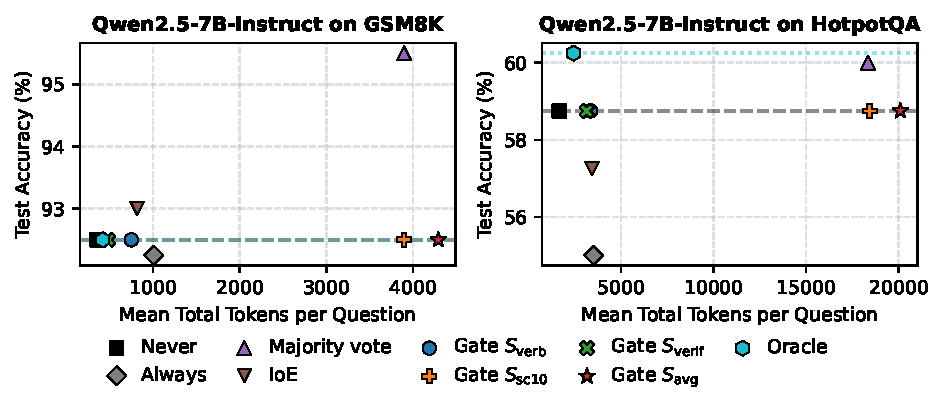
\includegraphics[width=\linewidth]{figure1_accuracy_cost.pdf}
\caption{Accuracy versus compute cost (mean total tokens per question, prefill plus completion) across baseline and confidence-gated revision policies for \modelA{} on GSM8K and HotpotQA. Dashed lines indicate the Never-revise baseline and the Oracle ceiling.}
\label{fig:cost}
\label{fig:accuracy_cost}
\end{figure}

Figure~\ref{fig:cost} relates accuracy to the mean number of tokens per question. The methods fall into two cost groups. Never revising costs about 350 tokens per GSM8K question and about 1{,}660 per HotpotQA question; self-critique, IoE, verbalized confidence and P(True) add roughly one more pass over the conversation. Everything based on self-consistency---the $S_{\text{sc}}$ gates and majority voting---needs about eleven times the tokens of a single answer, because ten full answers are sampled. P(True) generates only a single token, but on HotpotQA it re-reads all ten paragraphs and roughly doubles the prompt tokens (about 3{,}000 instead of 1{,}500). The accuracy gains of majority voting therefore come at a substantial cost.

\section{Analysis}
\label{sec:analysis}

\subsection{Does the Analytical Model Predict Gated Accuracy?}
\label{sec:assumption}
With self-critique as the revision step, the development-tuned gates revise almost no questions, so their operating points $(u,t)$ lie close to the origin and Eq.~\eqref{eq:gated} reproduces the observed accuracies trivially (Table~\ref{tab:model_check} in Appendix~\ref{app:full}). The ceiling is the informative prediction here: no gate can improve on never revising by more than $(1-a)f$, which is 0 points on GSM8K and 1.5 points on HotpotQA, and no gate does. Majority voting as the revision step provides a non-trivial test, because its gates revise about 9\% of the HotpotQA questions. Inserting the measured $a$, $f_{\text{mv}}$, $b_{\text{mv}}$ and the gate's $(u,t)$ into Eq.~\eqref{eq:gated} predicts 59.56\% for the $S_{\text{sc}}$ gate and 59.58\% for the $S_{\text{avg}}$ gate; the observed accuracy is 59.50\% for both (Table~\ref{tab:mv}). The independence assumption of Section~\ref{sec:theory} thus appears adequate at this scale.

\subsection{Anatomy of Harmful Revisions}
\begin{table}[ht]
\centering
\caption{Analysis of harmful revisions ($R\to W$) under always-revise on HotpotQA ($N=400$). Comparing exact match (EM) against lenient string containment reveals how many apparent errors arise from surface format drift rather than semantic loss.}
\label{tab:format_drift}
\begin{tabular}{lccc}
\toprule
Model & Always-Revise $R\to W$ (EM) & Always-Revise $R\to W$ (Lenient) & Format Drift Cases \\
\midrule
\modelA{} & 21 & 17 & 4 \\
\bottomrule
\end{tabular}

\end{table}

The main reason why gating cannot help with self-critique is that the revision step rarely changes anything. On GSM8K, the revised answer differs from the initial one for only 2 of 500 questions, and for only 1 of the 38 questions whose initial answer is wrong. Reading these cases shows that the model re-checks its solution and confirms it, even when it is wrong. For question \texttt{gsm8k-test-255} (gold answer 192), the initial solution computes $8 \times 12 = 96$ cows; the revision repeats the same step and ends with ``Upon review, the steps are correct.'' On HotpotQA, revision changes 11.4\% of the answers, but these changes break more answers than they fix. Under lenient matching, 4 of the 21 HotpotQA $R\to W$ cases are no longer counted as errors, so part of the apparent harm is a change in answer form rather than in content. Score histograms and threshold-sensitivity curves are given in Appendix~\ref{app:full}.

\section{Discussion}
\label{sec:discussion}

\paragraph{The bottleneck is the revision, not the gate.} The analytical model separates two questions that are easy to confuse: whether revising helps on the questions it touches, measured by the fix and break rates, and whether a confidence signal can find those questions, measured by its ROC curve. Our results show that the first question decides the outcome. With self-critique, the fix rate is zero on GSM8K and very small on HotpotQA, so no signal can make revision useful, even though self-consistency identifies wrong answers well. With majority voting as the revision step, the same signals and the same gates produce gains that match the model's prediction. A gate can remove harm, but it cannot create fixes.

\paragraph{Why self-critique fails here.} The revised answers show a clear pattern of self-confirmation: the model repeats its earlier reasoning and declares it correct. Part of this is probably caused by our revision prompt, which explicitly allows the model to keep its answer when it finds no error. A more critical prompt might raise the fix rate, but, as the HotpotQA results suggest, it would probably raise the break rate as well. Measuring both rates is more informative than reporting net accuracy alone.

\paragraph{Answers to the research questions.} \textbf{RQ1:} With self-critique as the revision step, no gate outperforms never revising; with majority voting as the revision step, gating keeps most of the benefit of majority voting while revising far fewer questions, but its advantage over never revising is not significant on our test sets, and a small development split can fail to find a useful threshold. \textbf{RQ2:} Self-consistency is the most discriminative signal (AUROC 0.95 on GSM8K and 0.69 on HotpotQA); verbalized confidence and P(True) are weak (0.58--0.64). \textbf{RQ3:} The best signal is also the most expensive: self-consistency needs about eleven times the tokens of a single answer, whereas P(True) is cheap to generate but expensive to prefill when the context is long.

\paragraph{Comparison with prior work.} Our always-revise results agree with Huang et al.~\cite{huang2024cannot}: without external feedback, revision does not improve reasoning accuracy and can reduce it. In the terms of Yang et al.~\cite{yang2024confidence}, \modelA{} shows high confidence (it rarely changes a correct answer) but very low critique ability (it almost never repairs a wrong one). IoE~\cite{li2024confidence} behaves like a cautious revision step: it changes few answers and, on HotpotQA, still breaks more than it fixes. The strength of majority voting is consistent with Wang et al.~\cite{wang2023selfconsistency}.

\paragraph{Practical recommendation.} Before adding a confidence gate to a self-correction pipeline, practitioners should estimate the fix and break rates of the revision step on a development set. If $(1-a)f$ is small, the expected benefit of any gate is small as well, and effort is better spent on a revision step that actually repairs errors, such as resampling, or on obtaining external feedback.

\section{Limitations}
\label{sec:limitations}

The study has several limitations that bound how far its conclusions reach.
\begin{itemize}
    \item \textbf{Models.} We study a single open instruction-tuned model with 7B parameters, so our conclusions may not transfer to other model families or sizes. Larger models are reported to judge their own answers more reliably~\cite{kadavath2022language} and may have different fix and break rates, so the ranking of signals could change with scale. The model was run in 16-bit floating point on T4 GPUs; small numerical differences from other hardware or precisions are possible.
    \item \textbf{Tasks.} Both tasks are in English and have short answers that can be checked automatically. Open-ended generation, where correctness needs a semantic judgement, is outside our scope.
    \item \textbf{Sample size.} Each dataset contributes a few hundred test questions. This is enough to compare methods with paired tests, but confidence intervals are wide, and small accuracy differences between gates should not be over-interpreted.
    \item \textbf{Prompts.} We use one critique-and-revise prompt and a single round of revision. Fix and break rates depend on the wording of the revision prompt~\cite{yang2024confidence}, so other prompts or multi-round revision could shift the results.
    \item \textbf{Labels.} Exact match can mark a correct but differently phrased answer as wrong. This adds noise to the correctness labels, to the transition counts and to AUROC. We quantify the effect with a lenient match on HotpotQA, but do not remove it.
    \item \textbf{Analytical model.} The model in Section~\ref{sec:theory} assumes that the outcome of revision is independent of the confidence score once correctness is known. Section~\ref{sec:assumption} tests how well this holds; where it fails, the model's predictions are only approximate.
    \item \textbf{Threshold selection.} The development split is small compared with the number of candidate thresholds, so the chosen threshold $\tau^*$ has sampling variance and may not be optimal on the test split.
    \item \textbf{Cost.} Token counts are a proxy for cost. Wall-clock time depends on hardware, batching and prefix caching, which can make repeated prefill much cheaper than our token counts suggest.
\end{itemize}

\section{Conclusion}
\label{sec:conclusion}

We asked when a language model should revise its own answer. Our analytical model shows that confidence gating can only help when the revision step actually repairs errors and the confidence signal is informative in the relevant region of its ROC curve. An uninformative signal can never beat the better of never and always revising, and the achievable gain is capped by the fix rate. Experiments with \modelA{} confirm both sides of this picture. Self-critique almost never repairs an error, so no gate improves on never revising, even though self-consistency identifies wrong answers well. When the majority answer of the self-consistency samples is used as the revision step instead, the same gates behave as the model predicts. For this reason, future work should focus on the revision step itself, and on selecting thresholds reliably from small development sets.

\bibliographystyle{unsrtnat}
\bibliography{references}
\raggedbottom
\appendix
\section{Prompts}
\label{app:prompts}
All prompts are given verbatim; \{...\} marks a placeholder filled per question. Each prompt is sent as a user turn with the model's own chat template.

\paragraph{A0 GSM8K}
\begin{lstlisting}
Solve the following problem step by step. At the end, write your answer on a new line as:
Final answer: <answer>

Problem: {question}
\end{lstlisting}

\paragraph{A0 HotpotQA}
\begin{lstlisting}
Answer the question using the paragraphs below. Think step by step. At the end, write your answer on a new line as:
Final answer: <answer>
The answer should be a short span (a name, date, number, or yes/no).

Paragraphs:
{context}

Question: {question}
\end{lstlisting}

\paragraph{Verbalized confidence}
\begin{lstlisting}
How confident are you that your final answer above is correct? Reply with a single integer from 0 to 100 and nothing else.
\end{lstlisting}

\paragraph{Self-verification P(True)}
\begin{lstlisting}
Question: {question}
Proposed answer: {extracted_A0_answer}
Is the proposed answer correct?
(A) True
(B) False
Answer with the letter only.
\end{lstlisting}
The assistant turn is prefilled with ``The proposed answer is: ('' and the next-token probabilities of ``A'' and ``B'' are read.

\paragraph{Revision}
\begin{lstlisting}
Review your previous answer carefully. Check each step for errors. If you find a specific error, correct it. If you find no error, keep your original answer. End with a new line: Final answer: <answer>
\end{lstlisting}

\paragraph{IoE}
\begin{lstlisting}
Review your previous answer. If you are very confident about your answer, maintain your answer. Otherwise, update your answer. End with a new line: Final answer: <answer>
\end{lstlisting}
Adapted from Li et al.~\cite{li2024confidence}.

\section{Implementation Details}
\label{app:implementation}
All experiments were run on Kaggle with two NVIDIA T4 GPUs (16\,GB each), using vLLM 0.6.6.post1 with tensor parallelism over both GPUs, PyTorch 2.5.1+cu121, Transformers 4.48.3, 16-bit floating point and a maximum context length of 4{,}096 tokens. Each of the ten self-consistency samples uses its own random seed (42--51). Before every full run, a dry run on 20 questions checked that the gold answer never appears in the verification prompt, that all stages are aligned by question identifier, that a random score yields an AUROC near 0.5, and that the self-consistency samples are diverse. No verbalized-confidence or P(True) output failed to parse on the dry runs. The code, prompts, data splits and raw outputs are available at \url{\repourl}; the README lists the exact commands to reproduce all tables and figures.

\section{Contribution Summary and Use of AI Tools}
\label{app:contribution}

\paragraph{Contribution summary.} This is individual work. The author formulated the research question, designed the study (the three confidence signals, the tasks, the four-way transition analysis, the dev/test protocol and the baselines), ran and monitored all experiments, checked the results, and is responsible for all claims in the paper.

\paragraph{Use of AI tools.} AI assistants were used for coding support in implementing the experiment pipeline, for help with drafting, restructuring and editing the text, and for checking bibliographic details. All AI-generated code and text were reviewed and revised by the author. No AI tool was used to produce data, labels or reported numbers; all results come from the logged experiment outputs in the repository~(\url{\repourl}).

\section{Complete Numerical Results across All Experimental Settings}
\label{app:full}
\label{app:full_results}

This appendix provides the complete tabular breakdown of accuracy, revision rates, transition frequencies ($W\to R$ and $R\to W$), token costs, and exact McNemar significance tests across all evaluated methods and confidence gates for \modelA{} on GSM8K and HotpotQA, as well as the analytical model verification, score distributions, and threshold sensitivity curves.

\subsection{Full Gating Results on GSM8K}
\label{app:tab_qwen_gsm8k}
\begin{table}[H]
\centering
\caption{Full gating results for \modelA{} on GSM8K ($N=400$ test questions).}
\label{tab:full_qwen_gsm8k}
\resizebox{\linewidth}{!}{\begin{tabular}{lccccccccc}
\toprule
Method & $\tau^*$ & Acc (\%) & Rev (\%) & $W\to R$ & $R\to W$ & Prompt Tok & Comp Tok & $p_{\text{Never}}$ & $p_{\text{Always}}$ \\
\midrule
Never & -- & 92.5 & 0.0 & 0 & 0 & 121 & 232 & -- & 1.00 \\
Always & -- & 92.3 & 100.0 & 0 & 1 & 528 & 479 & 1.00 & -- \\
Majority vote & -- & 95.5 & 5.5 & 14 & 2 & 1326 & 2570 & 0.004 & 0.002 \\
IoE & -- & 93.0 & 1.0 & 2 & 0 & 519 & 297 & 0.500 & 0.250 \\
\midrule
Gate $S_{\text{verb}}$ & 0.000 & 92.5 & 0.0 & 0 & 0 & 512 & 236 & 1.00 & 1.00 \\
Gate $S_{\text{verb}}$ (hindsight)$^\dagger$ & 0.000 & 92.5 & 0.0 & 0 & 0 & 512 & 236 & 1.00 & 1.00 \\
Gate $S_{\text{sc10}}$ & 0.000 & 92.5 & 0.0 & 0 & 0 & 1326 & 2570 & 1.00 & 1.00 \\
Gate $S_{\text{sc10}}$ (hindsight)$^\dagger$ & 0.000 & 92.5 & 0.0 & 0 & 0 & 1326 & 2570 & 1.00 & 1.00 \\
Gate $S_{\text{verif}}$ & 0.000 & 92.5 & 0.0 & 0 & 0 & 248 & 233 & 1.00 & 1.00 \\
Gate $S_{\text{verif}}$ (hindsight)$^\dagger$ & 0.000 & 92.5 & 0.0 & 0 & 0 & 248 & 233 & 1.00 & 1.00 \\
Gate $S_{\text{avg}}$ & 0.000 & 92.5 & 0.0 & 0 & 0 & 1717 & 2574 & 1.00 & 1.00 \\
Gate $S_{\text{avg}}$ (hindsight)$^\dagger$ & 0.000 & 92.5 & 0.0 & 0 & 0 & 1717 & 2574 & 1.00 & 1.00 \\
\midrule
Oracle & -- & 92.5 & 7.5 & 0 & 0 & 160 & 259 & 1.00 & 1.00 \\
\bottomrule
\multicolumn{10}{l}{\footnotesize $^\dagger$Oracle-tuned upper bound on test set (not a practical method).}\\
\end{tabular}
}
\end{table}

\subsection{Full Gating Results on HotpotQA}
\label{app:tab_qwen_hotpotqa}
\begin{table}[H]
\centering
\caption{Full gating results for \modelA{} on HotpotQA ($N=400$ test questions).}
\label{tab:full_qwen_hotpotqa}
\resizebox{\linewidth}{!}{\begin{tabular}{lccccccccc}
\toprule
Method & $\tau^*$ & Acc (\%) & Rev (\%) & $W\to R$ & $R\to W$ & Prompt Tok & Comp Tok & $p_{\text{Never}}$ & $p_{\text{Always}}$ \\
\midrule
Never & -- & 58.8 & 0.0 & 0 & 0 & 1510 & 149 & -- & 0.006 \\
Always & -- & 55.0 & 100.0 & 6 & 21 & 3223 & 301 & 0.006 & -- \\
Majority vote & -- & 60.0 & 11.5 & 13 & 8 & 16611 & 1726 & 0.383 & 0.002 \\
IoE & -- & 57.3 & 6.5 & 1 & 7 & 3214 & 222 & 0.070 & 0.108 \\
\midrule
Gate $S_{\text{verb}}$ & 0.000 & 58.8 & 0.0 & 0 & 0 & 3207 & 152 & 1.00 & 0.006 \\
Gate $S_{\text{verb}}$ (hindsight)$^\dagger$ & 0.000 & 58.8 & 0.0 & 0 & 0 & 3207 & 152 & 1.00 & 0.006 \\
Gate $S_{\text{sc10}}$ & 0.100 & 58.8 & 4.8 & 0 & 0 & 16701 & 1736 & 1.00 & 0.006 \\
Gate $S_{\text{sc10}}$ (hindsight)$^\dagger$ & 0.200 & 59.5 & 9.0 & 3 & 0 & 16701 & 1736 & 0.250 & 2.8e-04 \\
Gate $S_{\text{verif}}$ & 0.000 & 58.8 & 0.0 & 0 & 0 & 3004 & 150 & 1.00 & 0.006 \\
Gate $S_{\text{verif}}$ (hindsight)$^\dagger$ & 0.000 & 58.8 & 0.0 & 0 & 0 & 3004 & 150 & 1.00 & 0.006 \\
Gate $S_{\text{avg}}$ & 0.425 & 58.8 & 2.3 & 0 & 0 & 18351 & 1734 & 1.00 & 0.006 \\
Gate $S_{\text{avg}}$ (hindsight)$^\dagger$ & 0.575 & 59.5 & 10.5 & 3 & 0 & 18351 & 1734 & 0.250 & 2.8e-04 \\
\midrule
Oracle & -- & 60.3 & 41.3 & 6 & 0 & 2227 & 214 & 0.031 & 9.5e-07 \\
\bottomrule
\multicolumn{10}{l}{\footnotesize $^\dagger$Oracle-tuned upper bound on test set (not a practical method).}\\
\end{tabular}
}
\end{table}

\subsection{Analytical Model Verification}
\label{app:analytical_model}
\begin{table}[H]
\centering
\caption{Comparison of predicted gated accuracy from the analytical model (Eq.~\ref{eq:gated}) against empirically observed gated accuracy on the test set ($N=400$ per dataset).}
\label{tab:model_check}
\resizebox{\linewidth}{!}{\begin{tabular}{llccccccc}
\toprule
Model & Dataset & Gate & $\tau^*$ & TPR ($t$) & FPR ($u$) & Pred Acc (\%) & Obs Acc (\%) & Diff (\%) \\
\midrule
\modelA{} & GSM8K & $S_{\text{verb}}$ & 0.000 & 0.000 & 0.000 & 92.50 & 92.50 & +0.00 \\
\modelA{} & GSM8K & $S_{\text{sc10}}$ & 0.000 & 0.000 & 0.000 & 92.50 & 92.50 & +0.00 \\
\modelA{} & GSM8K & $S_{\text{verif}}$ & 0.000 & 0.000 & 0.000 & 92.50 & 92.50 & +0.00 \\
\modelA{} & GSM8K & $S_{\text{avg}}$ & 0.000 & 0.000 & 0.000 & 92.50 & 92.50 & +0.00 \\
\modelA{} & HotpotQA & $S_{\text{verb}}$ & 0.000 & 0.000 & 0.000 & 58.75 & 58.75 & +0.00 \\
\modelA{} & HotpotQA & $S_{\text{sc10}}$ & 0.100 & 0.103 & 0.009 & 58.86 & 58.75 & -0.11 \\
\modelA{} & HotpotQA & $S_{\text{verif}}$ & 0.000 & 0.000 & 0.000 & 58.75 & 58.75 & +0.00 \\
\modelA{} & HotpotQA & $S_{\text{avg}}$ & 0.425 & 0.055 & 0.000 & 58.83 & 58.75 & -0.08 \\
\bottomrule
\end{tabular}
}
\end{table}

\subsection{Score Distributions and Threshold Sensitivity}
\label{app:distributions_and_sensitivity}

\begin{figure}[H]
\centering
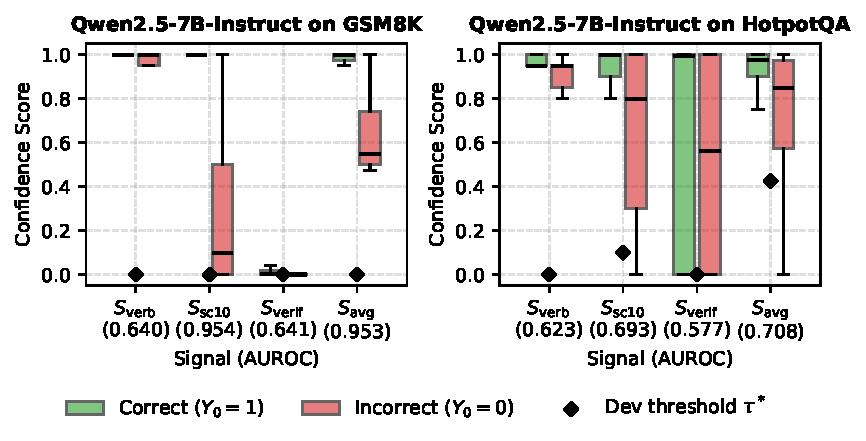
\includegraphics[width=0.9\linewidth]{figure2_histograms.pdf}
\caption{Distributions of confidence scores for correct ($Y_0=1$) versus incorrect ($Y_0=0$) initial answers across signals on GSM8K (left) and HotpotQA (right) for \modelA{}. Diamonds indicate the dev-selected threshold $\tau^*$.}
\label{fig:hist}
\label{fig:histograms}
\end{figure}

\begin{figure}[H]
\centering
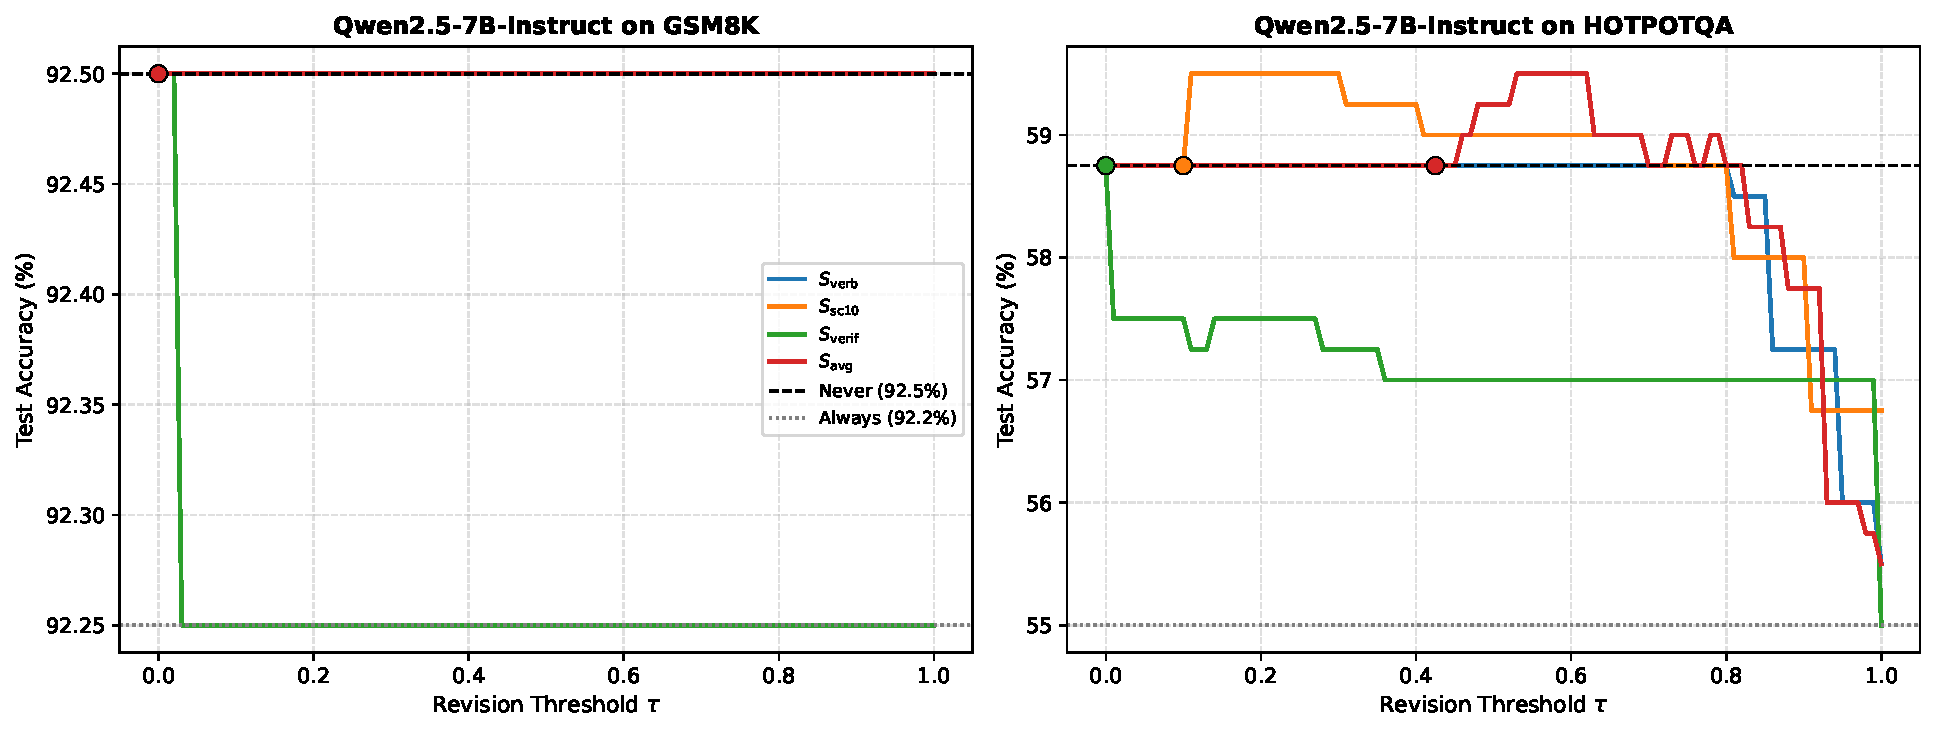
\includegraphics[width=0.9\linewidth]{figure3_tau_sensitivity.pdf}
\caption{Sensitivity of test accuracy to revision threshold $\tau$ for each confidence signal on GSM8K (left) and HotpotQA (right). Markers indicate operating points at the dev-selected threshold $\tau^*$.}
\label{fig:tau}
\label{fig:tau_sensitivity}
\end{figure}

% Declaration of Academic Integrity: the signed form (git-ignored) if present, else the pre-filled one
\clearpage
\IfFileExists{declaration/declaration_signed.pdf}
  {\includepdf[pages=-]{declaration/declaration_signed.pdf}}
  {
\includepdf[pages=-]{declaration/declaration_prefilled.pdf}}
\end{document}
